
\section{Máquinas virtuais versus {\conts}}

A virtualização, nomeadamente sob a forma de Máquinas Virtuais (VM), é uma tecnologia que se encontra presente 
em múltiplos sistemas em produção, particularmente em centros de dados. Esta tem progredido maioritariamente devido à sua vasta utilização no contexto empresarial. As primeiras ocorrências de virtualização surgiram na década de 60 e atualmente ainda se encontram em desenvolvimento \cite{7095802}.

No entanto, recentemente surgiram novas tecnologias de virtualização com a intro\-du\-ção dos  {\linconts} em 2008 \cite{wiki-lxc}. 
Esta nova tecnologia trouxe consigo uma solução mais leve em termos dos recursos exigidos, sacrificando isolamento e segurança.
 
Uma das soluções mais populares de virtualização por {\conts} é disponibilizada pela plataforma Docker \cite{docker} e executada num ambiente Linux. A figura \ref{fig:vms-conts}, retirada de \cite{image-vms-conts}, apresenta uma visualização sintética das duas tecnologias e das principais diferenças, que são em seguida apresentadas em mais detalhe.

\begin{figure}[h!]
	\centering
	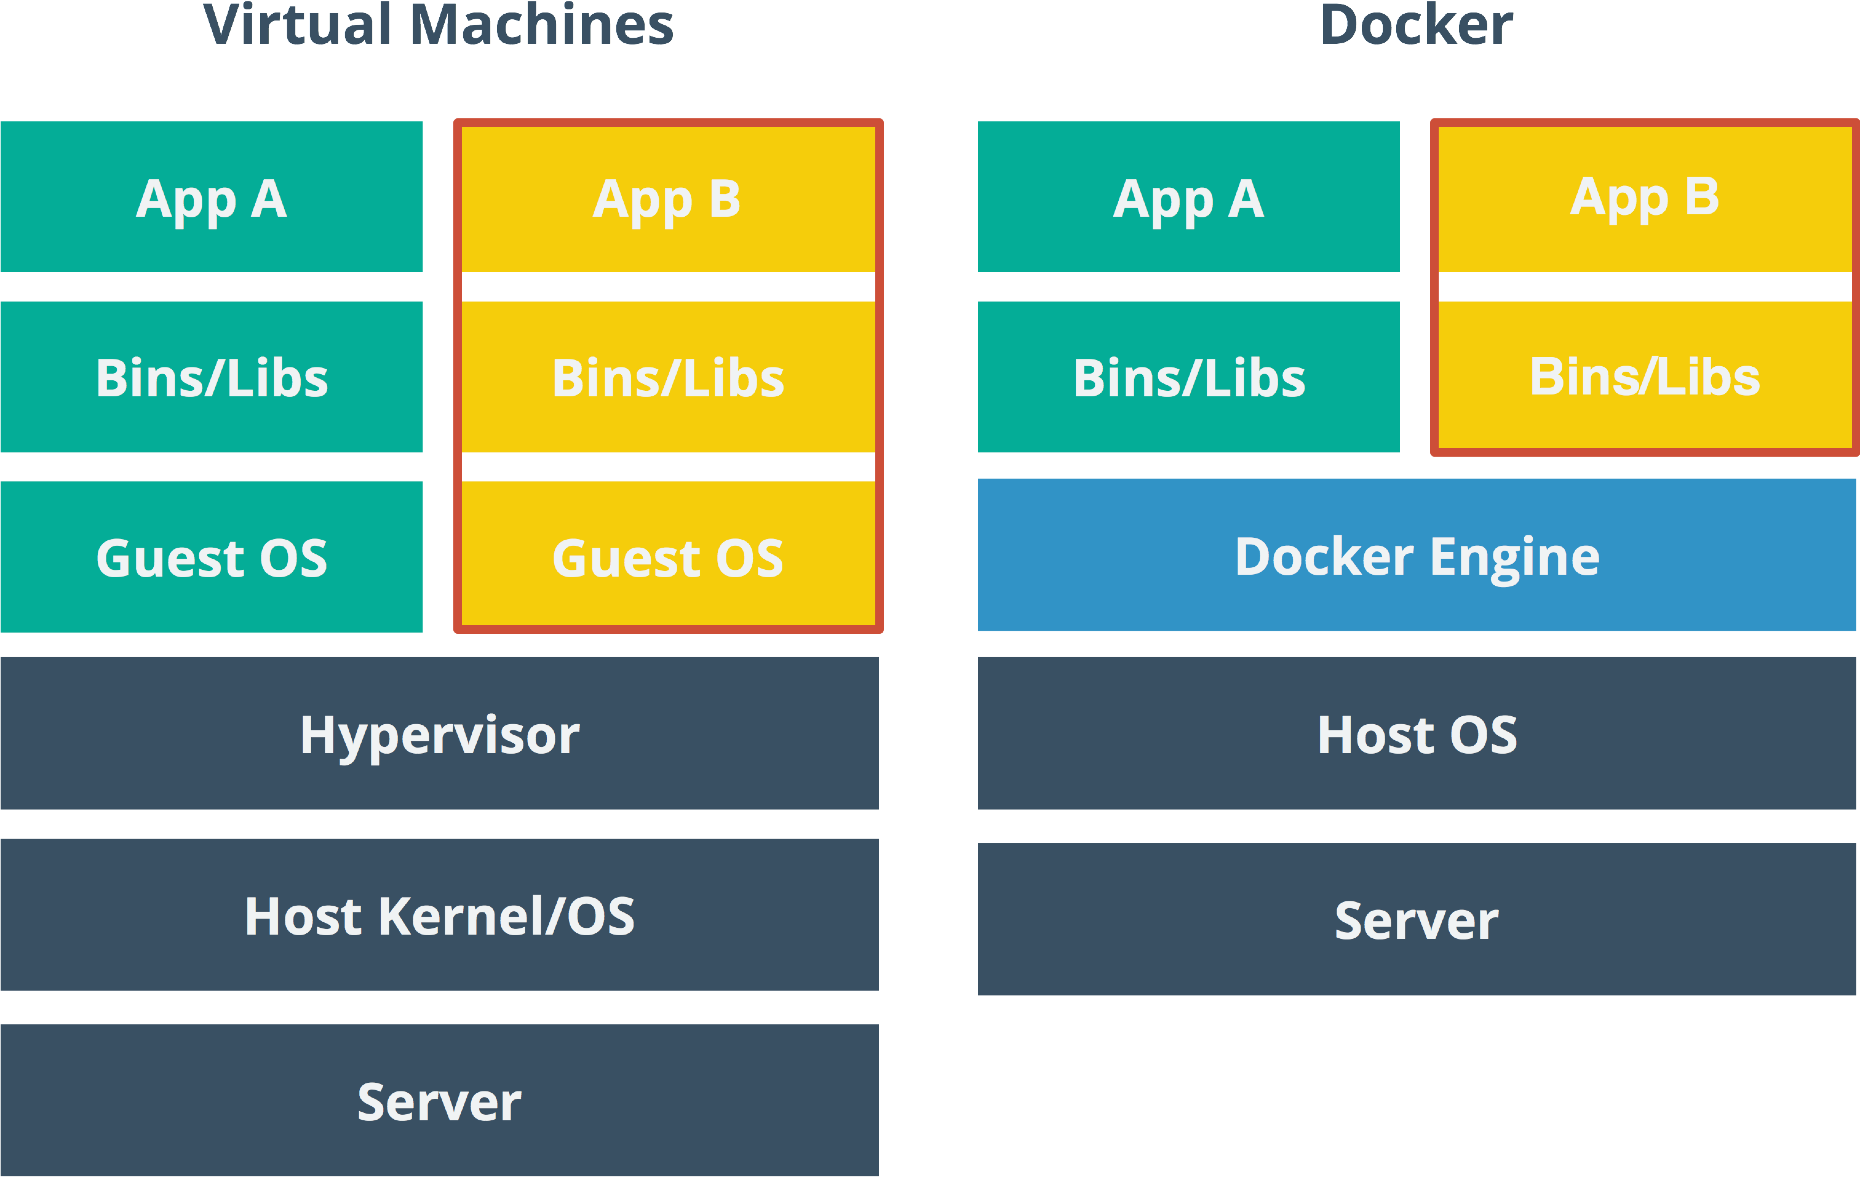
\includegraphics[width=\linewidth]{figures/docker-vs-virtual-machines.png}
	\caption{Arquitetura da virtualização em VMs e {\conts}} \cite{image-vms-conts}
	\label{fig:vms-conts}
\end{figure}


\subsection{Máquinas Virtuais}
Num ambiente de virtualização com recurso a máquinas virtuais o {\hiper} é o componente principal. Como podemos observar na figura \ref{fig:vms-conts}, este componente é fundamental pois é responsável por ocultar o \textit{hardware} real e disponibilizar sob a forma de \textit{hardware} virtual (que nalguns casos, mas não em todos, tem exatamente as mesmas propriedades que o real) os recursos afetados à máquina virtual. O isolamento entre máquinas virtuais é um ponto forte desta solução. Este isolamento garante (à partida) que se um serviço for comprometido, outras máquinas virtuais instanciadas no mesmo servidor, e até o próprio {\hiper} não serão também comprometidas. 

De uma forma simplificada, podemos dizer que a execução de aplicações numa VM decorre na sua maior parte sem intervenção do {\hiper}; 
contudo, a execução de certas instruções privilegiadas obriga à sua intervenção, o que contribui com algum \textit{overhead} na execução.

\subsection{{\Conts}} \label{section_conts}
A tecnologia dos {\conts} baseia-se numa virtualização ao nível do sistema de operação (SO), inicialmente baseada nos \textit{control groups} e \textit{kernel namespaces} presentes no Linux. Isto permite que várias instâncias de {\conts} possam ser executadas sobre o mesmo \textit{kernel}, evitando assim a camada de virtualização do \textit{hardware} presente nas máquinas virtuais (observável na Figura \ref{fig:vms-conts}). Assim, e ao contrário do que acontece nas VMs, a execução de tais instruções privilegiadas, {\eg} as utilizadas em leituras do disco, são efetuadas diretamente no SO do \textit{host}. A tecnologia Docker (\textit{Docker engine}) domina atualmente o mercado no que toca a este tipo de virtualização. No entanto a segurança da mesma ainda é um fator de preocupação devido à falta de isolamento entre processos. 

\discutir{rever isto, elaborar com a tabela, falar de Copy On write}

\begin{table}[h!]
\centering
    	\renewcommand{\arraystretch}{1.5}
	\setlength{\arrayrulewidth}{0.5mm}
	\setlength{\tabcolsep}{12pt}	
    \begin{tabular}{ | P{20mm} | P{40mm} | P{40mm} | } 
    \hline
    \textbf{Tópico} & \textbf{\Conts} & \textbf{Máquinas Virtuais} \\ \hline
    \hline
    \textbf{Virtualização} & Virtualização ao nível do sistema de operação & Virtualização ao nível do \textit{hardware} \\
    \hline
    \textbf{Inicialização} & Cerca de 500ms & Cerca de 20s \\
    \hline
    \textbf{Versatilidade} & Numa solução nativa é restrito ao ambiente Linux \footnotemark & Independente do sistema de operação \\
    \hline
    \textbf{Isolamento} & Baseado em \textit{namespaces} e \textit{Cgroups} & Isolamento total \\
    \hline
    \textbf{Maturidade da tecnologia} & Pouco empregue em contexto empresarial & Presente na maioria dos sistemas de virtualização em produção \\
    \hline
    \textbf{Chamadas de sistema} & Chamadas de sistema diretas ao SO do \textit{host} & Chamadas ao SO \textit{guest} e posteriormente ao {\hiper} \\
    \hline
    \textbf{Utilização de disco} & Apenas possui dependências dos executáveis e de um \textit{filesystem} & Possui todos os ficheiros presentes num sistema de operação \\
    \hline
\end{tabular}
\caption{Principais diferenças entre {\conts} e máquinas virtuais}
\end{table}


\footnotetext{O ambiente Docker está transportado para outros sistemas de operação mas geralmente recorre igualmente a máquinas virtuais, podendo ser considerada uma solução mista}

\subsection{Conclusões}

Em suma, as principais diferenças entre as duas opções de virtualização resumem-se no consumo de recursos por instância, isolamento entre instâncias e no nível de abstração. É importante salientar que, embora não sejam aspetos decisivos, o tempo de arranque, o espaço consumido em disco e ferramentas disponibilizadas pelas tecnologias {\eg} Docker Hub e VMWare vSphere são fatores a considerar ao escolher uma destas tecnologias.





